Moje drogie dzieci, po napisaniu historii rodziny Świerczyńskich postanowiłem ją dopełnić poprzez napisanie historii rodziny Głąbów, z której wywodzi się Wasza mama Czesława jako córka Franciszka Głąba i Eleonory z domu Mertówna. Franciszek Głąb, którego mieliście szansę poznać, przyszedł na świat 2~VIII 1910~r. w~Mirowie w~licznej już wówczas rodzinie Walentego i~Antoniny Głąbów. Ale dla porządku zacznijmy od najstarszej jego siostry Marianny...

Otóż Walenty Głąb ur. 29 I 1869~r. w~Mirowie (syn Macieja i Marianny z~Hamerlów) poślubił 12 IX 1894~r. we Włodowicach Antoninę Łyszczarzównę ur. 18 VI 1875~r. w~Górze Włodowskiej (córka Macieja i Józefy z domu Boniek lub Błońskiej, tak w akcie zgonu babci Antoniny), która wówczas była zupełną sierotą a jej prawnym opiekunem był Kacper Łyszczarz -- jej stryj (ryc.~\ref{rys:akt_slubu_walentego_glaba_i_antoniny_lyszczarz}).

\begin{figure}[!h]
\begin{center}
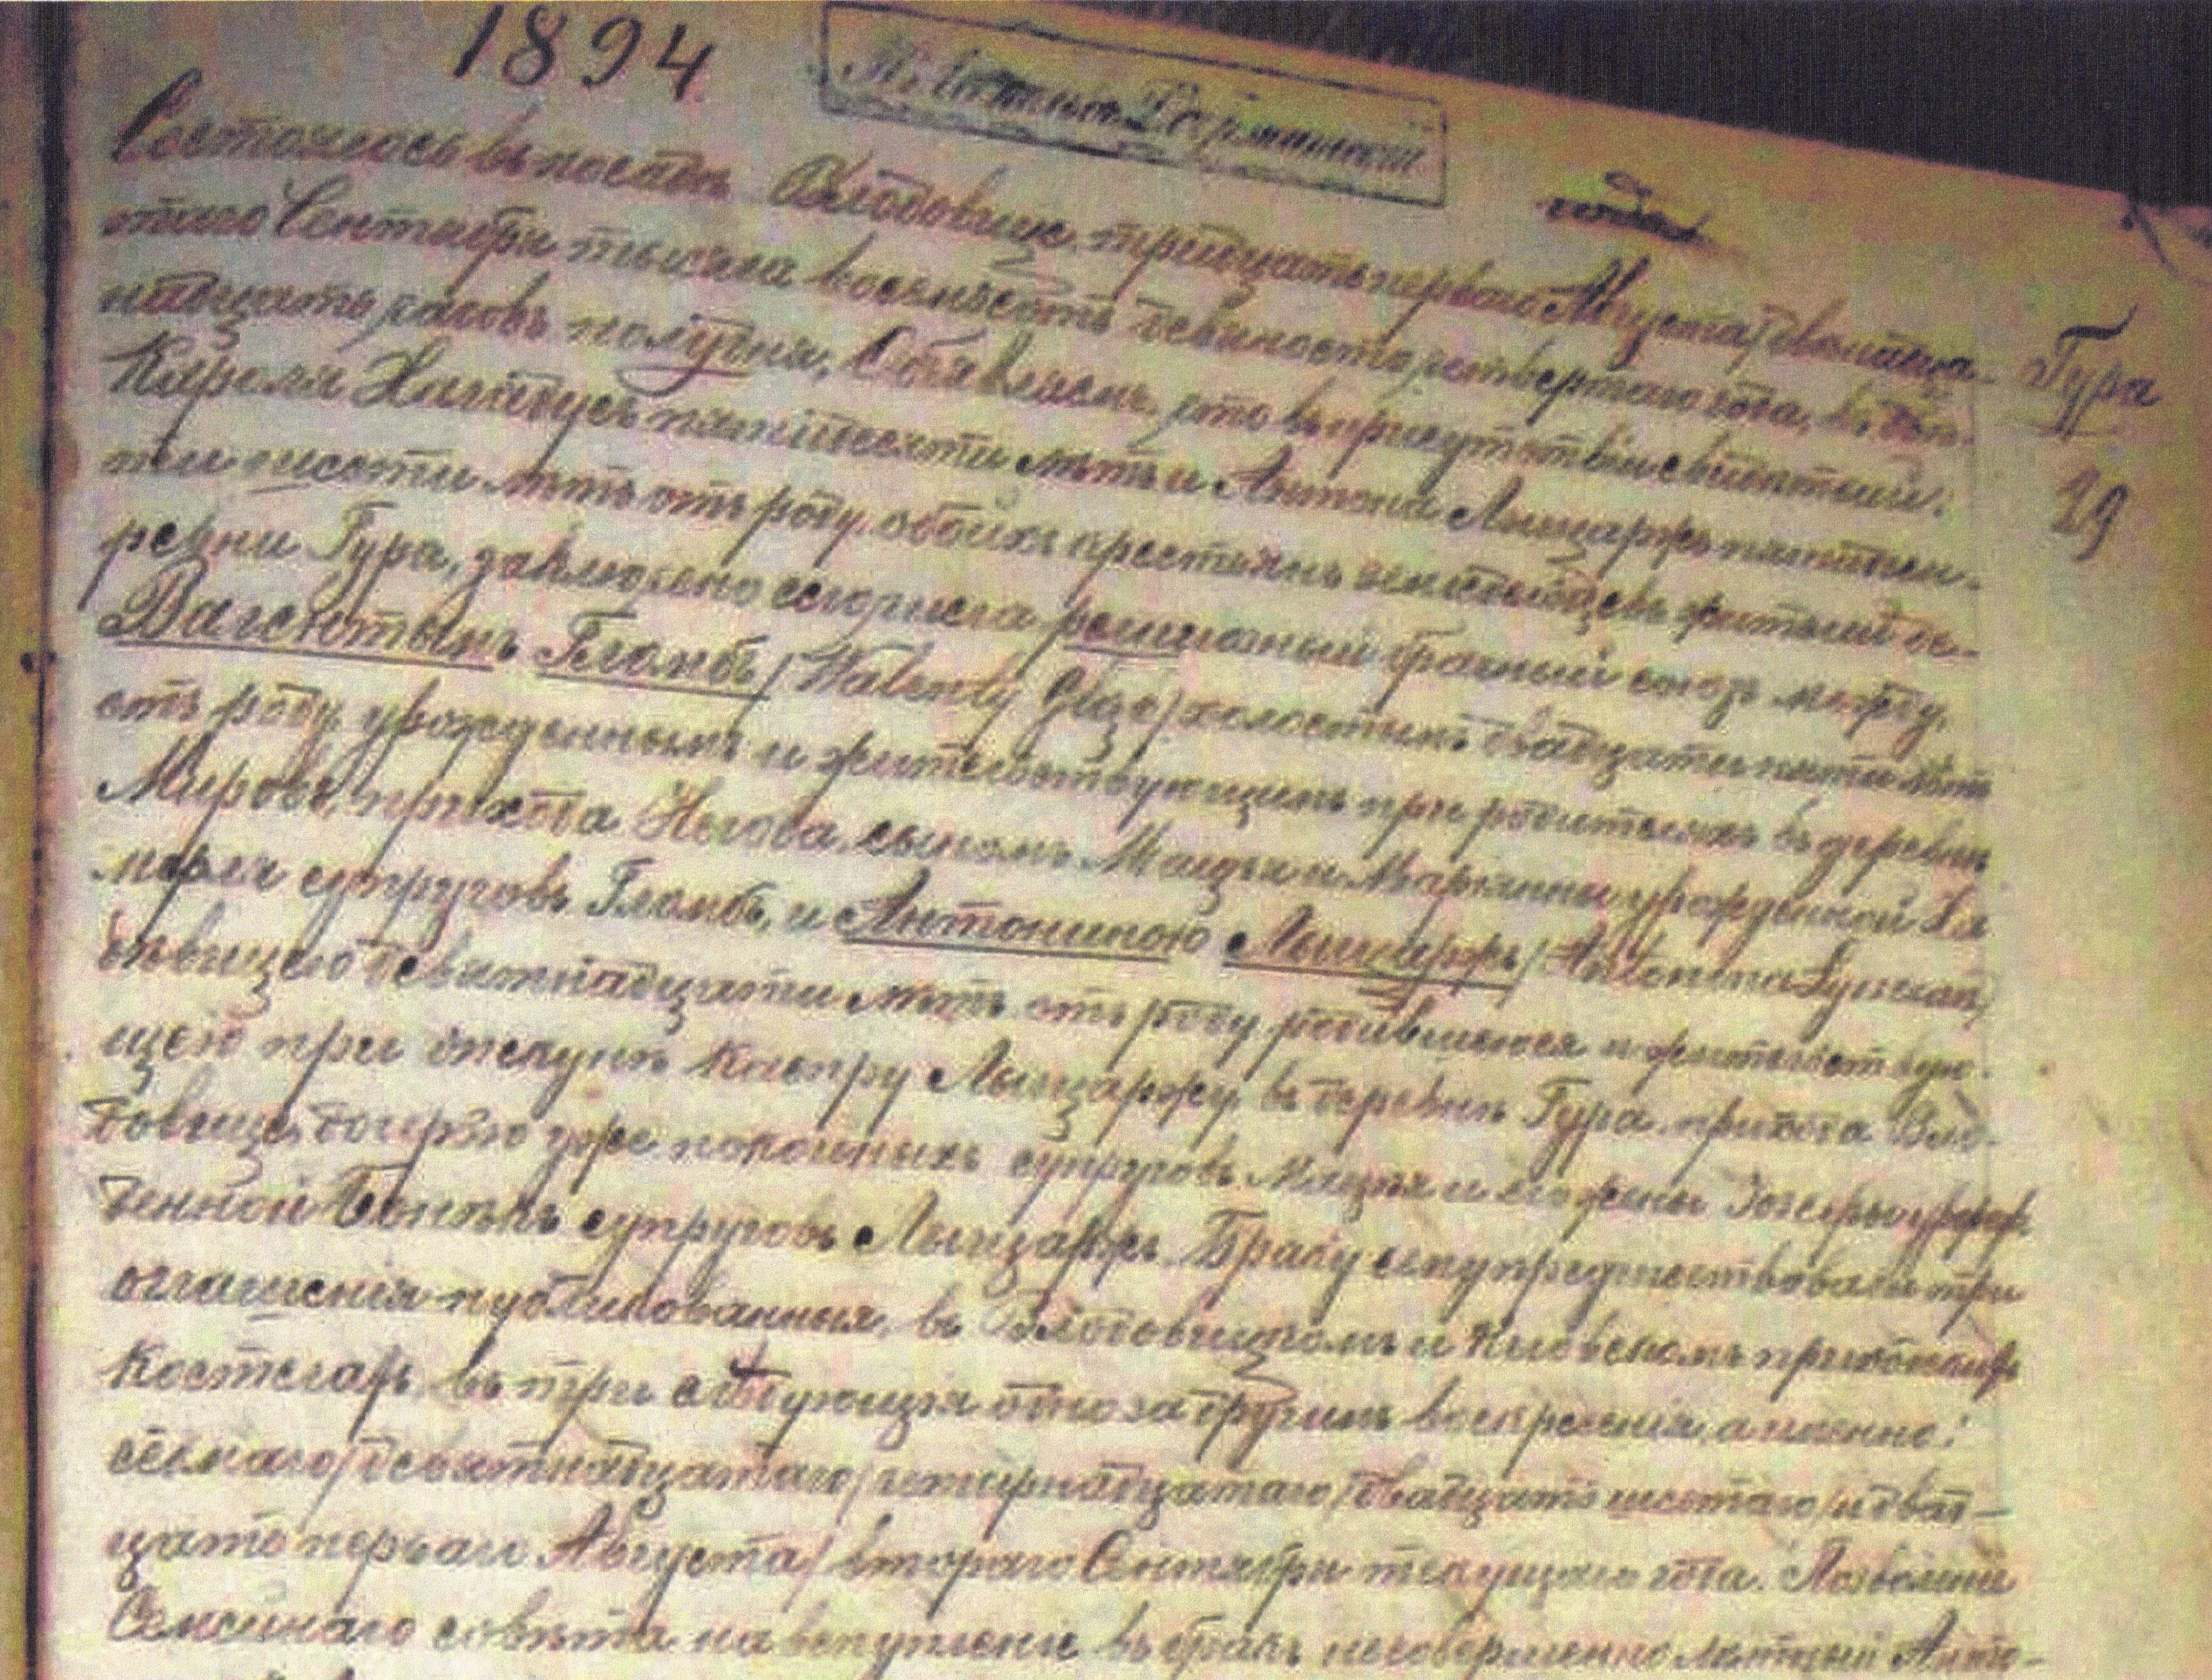
\includegraphics[width=0.9\textwidth]{zdjecia/akt_slubu_walentego_glaba_i_antoniny_lyszczarz.jpg}
\caption{Akt ślubu Walentego Głąba z Antoniną Łyszczarz.}
\label{rys:akt_slubu_walentego_glaba_i_antoniny_lyszczarz}
\end{center}
\end{figure}
